\documentclass[12pt,journal,compsoc]{IEEEtran}
\usepackage[spanish]{babel} % Para separar correctamente las palabras de multitud de idiomas
\usepackage[utf8]{inputenc} %Este paquete permite poner acentos directamente y eñes
\usepackage{graphicx}
\usepackage{caption}
\usepackage{float}
\usepackage{amsmath}
\usepackage[utf8]{inputenc}
\usepackage{url}
\usepackage{listings}
\ifCLASSINFOpdf
\else
\fi
\hyphenation{op-tical net-works semi-conduc-tor}
\usepackage{cite}
\usepackage{color}
\usepackage{graphicx}
\usepackage[justification=centering]{caption}

\lstset{
	language=C,                	   % choose the language of the code
	stepnumber=1,                   % the step between two line-numbers.        
  	numbersep=5pt,                  % how far the line-numbers are from the code
  	showspaces=false,               % show spaces adding particular underscores
  	showstringspaces=false,         % underline spaces within strings
  	showtabs=false,                 % show tabs within strings adding particular underscores
  	tabsize=5,                      % sets default tabsize to 2 spaces
  	captionpos=none,                   % sets the caption-position to bottom
  	breaklines=true,                % sets automatic line breaking
  	breakatwhitespace=true,         % sets if automatic breaks should only happen at whitespace
  	keywordstyle=\color{red},
  	basicstyle=\ttfamily\footnotesize,
  	title=\lstname,                 % show the filename of files included with \lstinputlisting;
}

\begin{document}
%
% paper title
% can use linebreaks \\ within to get better formatting as desired
% Do not put math or special symbols in the title.
\title{Simulación de carácter catastrófica del Sistema Solar en OpenGL}
%
%
% author names and IEEE memberships
% note positions of commas and nonbreaking spaces ( ~ ) LaTeX will not break
% a structure at a ~ so this keeps an author's name from being broken across
% two lines.
% use \thanks{} to gain access to the first footnote area
% a separate \thanks must be used for each paragraph as LaTeX2e's \thanks
% was not built to handle multiple paragraphs
%
%
%\IEEEcompsocitemizethanks is a special \thanks that produces the bulleted
% lists the Computer Society journals use for "first footnote" author
% affiliations. Use \IEEEcompsocthanksitem which works much like \item
% for each affiliation group. When not in compsoc mode,
% \IEEEcompsocitemizethanks becomes like \thanks and
% \IEEEcompsocthanksitem becomes a line break with idention. This
% facilitates dual compilation, although admittedly the differences in the
% desired content of \author between the different types of papers makes a
% one-size-fits-all approach a daunting prospect. For instance, compsoc 
% journal papers have the author affiliations above the "Manuscript
% received ..."  text while in non-compsoc journals this is reversed. Sigh.

\author{Wladimir Albornoz,~\IEEEmembership{estudiante, Usach} y Andrés Barrera,~\IEEEmembership{estudiante, Usach}}% <-this % stops a space

% note need leading \protect in front of \\ to get a newline within \thanks as
% \\ is fragile and will error, could use \hfil\break instead.Facultad de Ciencias.


% note the % following the last \IEEEmembership and also \thanks - 
% these prevent an unwanted space from occurring between the last author name
% and the end of the author line. i.e., if you had this:
% 
% \author{....lastname \thanks{...} \thanks{...} }
%                     ^------------^------------^----Do not want these spaces!
%
% a space would be appended to the last name and could cause every name on that
% line to be shifted left slightly. This is one of those "LaTeX things". For
% instance, "\textbf{A} \textbf{B}" will typeset as "A B" not "AB". To get
% "AB" then you have to do: "\textbf{A}\textbf{B}"
% \thanks is no different in this regard, so shield the last } of each \thanks
% that ends a line with a % and do not let a space in before the next \thanks.
% Spaces after \IEEEmembership other than the last one are OK (and needed) as
% you are supposed to have spaces between the names. For what it is worth,
% this is a minor point as most people would not even notice if the said evil
% space somehow managed to creep in.



% The paper headers
\markboth{Proyecto de Computación Grafica, 2do. Semestre de 2015}%
{Shell \MakeLowercase{\textit{et al.}}: Bare Advanced Demo of IEEEtran.cls for Journals}
% The only time the second header will appear is for the odd numbered pages
% after the title page when using the twoside option.
% 
% *** Note that you probably will NOT want to include the author's ***
% *** name in the headers of peer review papers.                   ***
% You can use \ifCLASSOPTIONpeerreview for conditional compilation here if
% you desire.



% The publisher's ID mark at the bottom of the page is less important with
% Computer Society journal papers as those publications place the marks
% outside of the main text columns and, therefore, unlike regular IEEE
% journals, the available text space is not reduced by their presence.
% If you want to put a publisher's ID mark on the page you can do it like
% this:
%\IEEEpubid{0000--0000/00\$00.00~\copyright~2012 IEEE}
% or like this to get the Computer Society new two part style.
%\IEEEpubid{\makebox[\columnwidth]{\hfill 0000--0000/00/\$00.00~\copyright~2012 IEEE}%
%\hspace{\columnsep}\makebox[\columnwidth]{Published by the IEEE Computer Society\hfill}}
% Remember, if you use this you must call \IEEEpubidadjcol in the second
% column for its text to clear the IEEEpubid mark (Computer Society journal
% papers don't need this extra clearance.)



% use for special paper notices
%\IEEEspecialpapernotice{(Invited Paper)}



% for Computer Society papers, we must declare the abstract and index terms
% PRIOR to the title within the \IEEEtitleabstractindextext IEEEtran
% command as these need to go into the title area created by \maketitle.
% As a general rule, do not put math, special symbols or citations
% in the abstract or keywords.
\IEEEtitleabstractindextext{%
\begin{abstract}
En el siguiente informe se detallan los aspectos preliminares para el proyecto de la asignatura de computación Gráfica, en este se presenta el modelamiento de sistema solar con un cinturón de asteroides, todo esto en un sistema de software. Otras implementaciones realizadas en este trabajo fueron la aplicación de texturas en el fondo de la escena utilizando la técnica de SkyBox y la implementación de un menú para facilitar la navegación entre las funcionalidades del programa y el experimento. Fue implementado en OpenGL bajo el sistema operativo GNU/Linux.
\end{abstract}

% Note that keywords are not normally used for peerreview papers.
\begin{IEEEkeywords}
Sistema solar, OpenGL, rotación, traslación, objetivos, herramientas a utilizar, plan.
\end{IEEEkeywords}}


% make the title area
\maketitle


% To allow for easy dual compilation without having to reenter the
% abstract/keywords data, the \IEEEtitleabstractindextext text will
% not be used in maketitle, but will appear (i.e., to be "transported")
% here as \IEEEdisplaynontitleabstractindextext when compsoc mode
% is not selected <OR> if conference mode is selected - because compsoc
% conference papers position the abstract like regular (non-compsoc)
% papers do!
\IEEEdisplaynontitleabstractindextext
% \IEEEdisplaynontitleabstractindextext has no effect when using
% compsoc under a non-conference mode.


% For peer review papers, you can put extra information on the cover
% page as needed:
% \ifCLASSOPTIONpeerreview
% \begin{center} \bfseries EDICS Category: 3-BBND \end{center}
% \fi
%
% For peerreview papers, this IEEEtran command inserts a page break and
% creates the second title. It will be ignored for other modes.
\IEEEpeerreviewmaketitle



\section{Introducción}
\IEEEPARstart{L}a idea principal del proyecto es generar una simulación de lo que pasaría si el Sol absorbiera a los planetas del sistema solar, fundamentalmente si se rompiera la resistencia existente, debido a que el sol se transformará en una gigante roja esto sucederá dentro de 10 mil millones de años aproximadamente \cite{Baker2015}. \\
Esta simulación tiene un carácter científico, ya que está demostrado que cuando se concrete el fin del sol terminaría absorbiendo a los planetas que se encuentren cercanos a el, se toman como base las diferentes visiones e información que se tiene del espacio-tiempo.\\
Debe considerarse que lo que se está presentando toma como base parte de un proyecto ya implementado \cite{anterior}, cabe destacar que esto resulta mas complejo debido a que la base está realizado con aspectos, métodos, módulos y herramientas diferentes, teniendo que considerar un tiempo extra para injertar de manera perfecta esto a el proyecto que se está realizando.
\section{Objetivos}
\subsection{Objetivo General}
Implementar gráficamente la simulación catastŕofica del sistema solar y que se aprecie lo mas apegado a la realidad posible.\\
\subsection{Objetivos Específicos}
\begin{itemize}
\item Conocer y relacionar términos de la computación gráfica para el desarrollo del proyecto \cite{foley}.
\item Entender y aprender a utilizar OpenGL para la implementación y representación de elementos de la computación gráfica.
\item Determinación de herramientas útiles para el desarrollo.
\item Descubir librerías que puedan ayudar tanto en la codificación como en la implementación.
\item Lograr dominar el lenguaje y las herramientas a utilizar.
\end{itemize}

\section{Descripción de la problemática}
\subsection{Motivación}
Resulta muy interesante la oportunidad de generar una simulación gráfica el sistema solar \cite{astronomia} conocido (figura \ref{planetas}), mas detalladamente del fin de el sol como se conoce, debido a la importancia que este sistema tiene para toda la humanidad; la mayor motivación para el desarrollo es en efecto poder implementar el proyecto, además con ello se pretende aprender y a la vez poner en práctica conceptos de la computación gráfica como la rotación, traslación y el modelado en 3 dimensiones.\\
\begin{figure}[h!]
  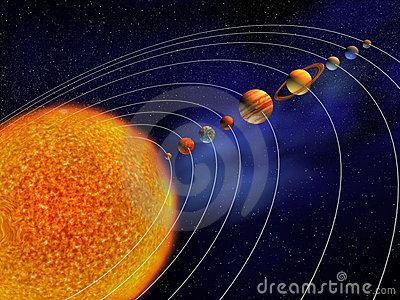
\includegraphics[width=0.45\textwidth]{planetas.jpg}
  \caption{Sistema solar conocido}
  \captionsetup{justification=centering}
  \label{planetas}
\end{figure}
\subsection{Definición de la problemática}
La mayoría de las implementaciones gráficas conocidas muestran simulaciones de la realidad de los planetas y del sistema solar, sus trayectorias, sus lunas o las diferencias entre las velocidades de rotación de cada uno; pero ¿que sucedería si las órbitas de los planetas aumentara y sumados al aumento de la masa del sol, este atrajera a todos los planetas existentes en el sistema conocido?, el fin de el sol y de los planetas como los conocemos es lo que se desea implementar.\\
Skybox es una tecnica que permite que una escena se vea más grande y más impresionante, envolviendo al usuario con una textura que es posible apreciar en una cámara de 360$^{\circ}$\cite{skybox2}.
\begin{figure}[h!]
  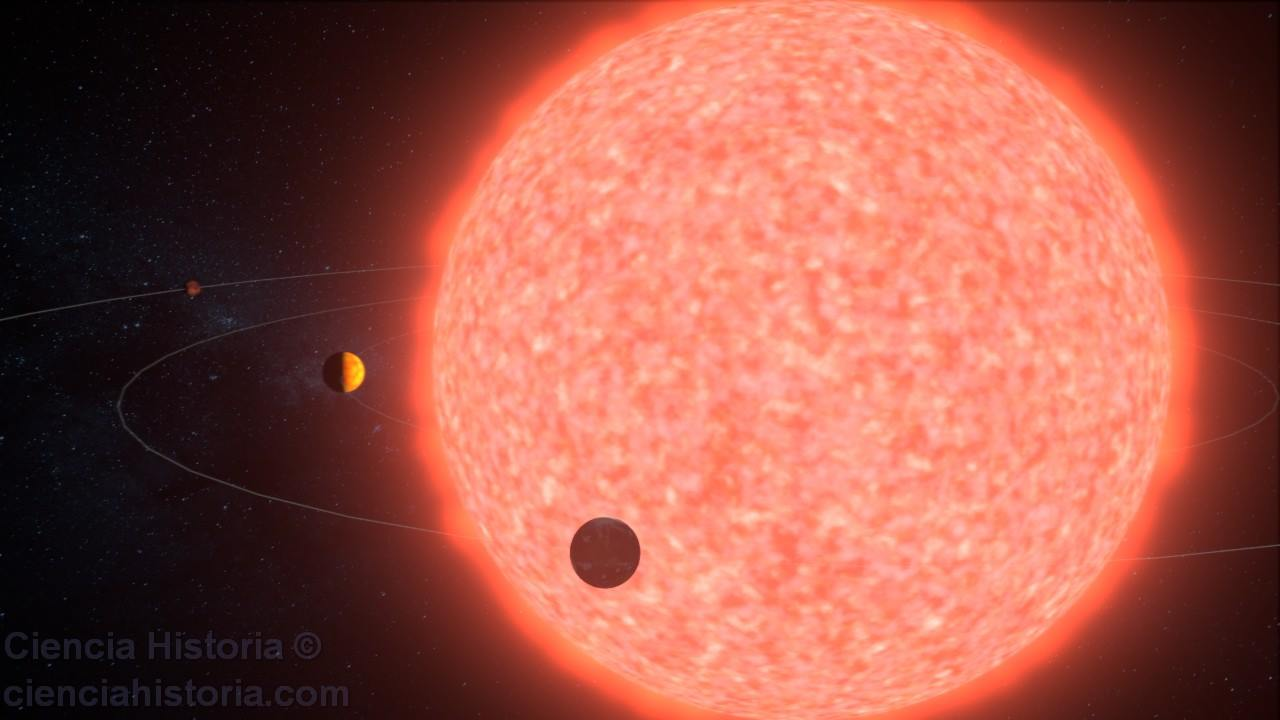
\includegraphics[width=0.48\textwidth]{sol.jpg}
  \caption{El Sol convertido en gigante roja llegando casi a la órbita de Venus, la Tierra tiene un futuro incierto}
  \captionsetup{justification=centering}
  \label{muerte}
\end{figure}
\section{Descripción de la solución propuesta}
Tomando como base el proyecto que solo muestra una representación del sistema solar, se pretende que la representación de las trayectorias de los planetas sea automática, con esto se refiere a que se vea el movimiento continuo de la trayectoria de los planetas y que eventualmente de a poco los planetas comiencen a cambiar su trayectoria, los cuales sumados al aumento del diámetro del sol, como se muestra en \ref{muerte}, empiecen a ser absorbidos por este, lo cual los hará desaparecer\cite{far}.\\
Para ello habría que:
\begin{itemize}
 \item Modificar algunas funciones relacionadas con la traslación de estas diferentes figuras (diferentes planetas)
 \item Editar y acondicionar las formulas de elipse.
 \item Aumentar el radio del sol.
\end{itemize}   %funcion %imagen de traslacion de planetas
\section{Modelamiento}
\subsection{Función de la elipse}
A continuación en la figura \ref{Elipse} se puede ver una elipse para posteriormente analizar su función matemática:
\begin{figure}[h!]
  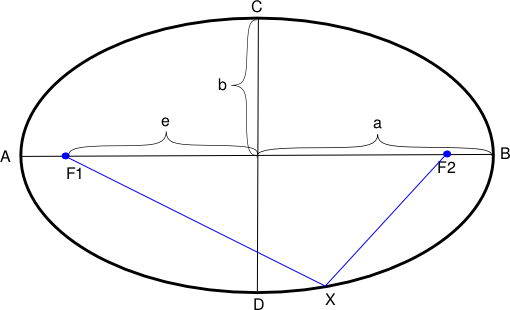
\includegraphics[width=0.48\textwidth]{Elipse.png}
  \caption{Elipse}
  \captionsetup{justification=centering}
  \label{Elipse}
\end{figure}

Se utiliza la función de la elipse:
\begin{huge}
\begin{center}
$\frac{x^{2}}{a^{2}} + \frac{y^{2}}{b^{2}}$
\end{center}
\end{huge}
Donde $a>0$ y $b>0$, las coordenadas de las abscisas. La elipse se encuentra centrada en el origen (h, k = 0). La ecuación de la elipse modela la ubicación de la órbita de los planetas.
\subsection{Transformaciones 3d}
Se utilizan una serie de trasnformaciones en el desarrollo del problema, estas seran mostradas a continuación:
\subsubsection{Rotación}
Claramente como se desea implementar un sistema solar, un detalle importante a destacar es la rotación que tiene cada planeta; la rotación está definida por la siguiente matriz:
\begin{center}
$
\begin{bmatrix}
cos\theta & -sin\theta \\
sin\theta & cos\theta 
\end{bmatrix}
$
\end{center}
En vista de que se trabaja en tres dimensiones es necesario definir las matrices para cada tipo de rotación que se pueden obtener desde la matriz de rotacion general de 2x2:\\
Rotación sobre el eje x:\\
\[
	R_{xy}(\theta) = \left[ 
		\begin{array}{cccc}
			1 & 0 & 0 & 0 \\
			0 & \cos\theta & -\sin\theta & 0 \\
			0 & \sin\theta & \cos\theta & 0 \\
			0 & 0 & 0 & 1
		\end{array}
	\right]
\]
Rotación sobre el eje y:\\
\[
	R_{yz}(\theta) = \left[ 
		\begin{array}{cccc}
			\cos\theta & 0 & \sin\theta & 0 \\
			0 & 1 & 0 & 0 \\
			-\sin\theta & 0 & \cos\theta & 0 \\
			0 & 0 & 0 & 1
		\end{array}
	\right]	
\]
Rotación sobre el eje z:\\
\[
	R_{zx}(\theta) = \left[ 
		\begin{array}{cccc}
			\cos\theta & -\sin\theta & 0 & 0 \\
			\sin\theta & \cos\theta & 0 & 0 \\
			0 & 0 & 1 & 0 \\
			0 & 0 & 0 & 1
		\end{array}
	\right]	
\]

Se describe como rotación en los planos $xy$, $yz$ y $zx$, pues resulta más fácil asociar la rotación en 3 dimensiones de esa forma. La órbita de los planetas se genera aplicando una rotación sobre el eje $y$ (En el origen, teniendo el solo como referencia) con un ángulo $0^{\circ}\leq\theta\leq360^{\circ}$, el cual aumenta en cada frame de la escena.
\subsubsection{Traslación}
La matriz que describe la traslación de los objetos en la escena es la siguiente:\\

\[ 
	T = \left[ 
			\begin{array}{cccc}
				1 & 0 & 0 & T_{x} \\
				0 & 1 & 0 & T_{y} \\
				0 & 0 & 1 & T_{z} \\
				0 & 0 & 0 & 1 
			\end{array}
		\right] \times 
		\left[ 
			\begin{array}{c}
				v_{x} \\
				v_{y} \\
				v_{z} \\
				v_{w} 
			\end{array}
		\right] = 
		\left(
			\begin{array}{ccc}
				v'_{x} , & v'_{y} , & v'_{z}
			\end{array}
		\right)
\]
La traslación permite saber el radio que tendrá la órbita del planeta respecto al sol. Es en torno a esta transformación que se aplica la rotación, por lo tanto para cada frame de la escena se aplica un pequeño aumento en la rotación respectiva.\\
\subsection{Distancia entre dos puntos}
Esta fórmula se utiliza para determinar la distancia entre 2 puntos en un plano en 2D, aunque el sistema está representado en 3 dimensiones. Los planetas se mueven respecto al eje y y la posición de los mismos está determinada sólo por sus coordenadas en el eje x y en el eje z:\\
\[ 
	x_{new} = \frac{\sqrt{X_{final}^{2}+X_{inicial}^{2}}}{100} 
\]
\newline
\[
	z_{new} = \frac{\sqrt{Z_{final}^{2}+Z_{inicial}^{2}}}{100}
\]
\newline
la distancia total entre el punto final y el inicial es dividida por un número random con ello se genera la traslación de un objeto desde un punto hacía otro; lo que se traslada es la viewport
\section{Diseño del problema}
A continuación, se especifica un diseño preliminar mas un diseño detallado del problema y de la solución
\subsection{Diseño preliminar}
La formulación del modelo en base al sistema solar y a la teoría del fin del sol en aproximadamente 10.000 millones de años aprox. es un modelo, debido a que los cálculos realizados son a escala respecto al sistema solar real, es decir, X pixeles son equivalentes a algunos años luz. Los tamaños de los planetas también son a escala, los tamaños de cada uno son equivalentes a la vida real, así también su color y movimiento.
\\
Dado esto, en pocas palabras seria de la siguiente forma:
\begin{itemize}
 \item Calcular la trayectoria de los planetas alrededor del sol
 \item Implementar un menú que permita navegar entre las
 distintas funcionalidades presentes en el programa
 \item Aplicar la técnica de SkyBox en la escena
\end{itemize}
\subsection{Diseño detallado}
OpenGl es el principal entorno de desarrollo, para la creación de aplicaciones graficas portátiles e interactivas en  2D y 3D. 
La API se suele utilizar para interactuar con una unidad de procesamiento gráfico (GPU), para lograr la aceleración por hardware de renderizado.
Desde su introducción en 1992, OpenGl se ha convertido en la Interfaz de Programación de Aplicaciones (API) gráficas más usada por la industria, brindando miles de aplicaciones a una gran variedad de plataformas de computación. A su vez, OpenGL fomenta la innovación y velocidad del desarrollo de aplicaciones incorporando una alta variedad de formas de rendering, mapeo de texturas, efectos especiales y otras poderosas funciones de visualización\cite{opengl}.
\\
Se utilizo el Entorno de Desarrollo Integrado (IDE) llamado NetBeans, el cual permite detectar rápidamente errores de sintaxis. Permite también iniciar en modo debug, herramienta con la cual es posible realizar un seguimiento del valor de cada variable en cada frame de la aplicación. Además, resulta mucho más fácil el proceso de compilación, ya que es un proceso mas gráfico que la ejecucion en una consola, además no discrimina el sistema operativo a ocupar.\\
\\
OpenGL trabaja con una pila de matrices, las cuales representan cada objeto que se muestra en la escena. A continuación se detallará el trabajo y la sintaxis de cada una de ellas.
%
\lstinputlisting{ejemplo.c} 
%
Extracto de código que nos permite demostrar cuando se crea una nueva matriz\\
Las transformaciones se aplican en un orden predefinido, es decir, primero se realiza la traslación (Desde el origen hacía el punto $(x,y,z)$) para posteriormente realizar la rotación sobre el eje deseado.Esto es apoyado por la literatura y la cátedra.\\
\\
Las transformaciones geométricas en OpenGL están implementadas, a continuación se mostraran en mas detalle cada una de ellas:
%
\subsubsection{Rotación}
\label{rotacion}
Para rotar, en openGL se utiliza la función \textbf{glRotate}, la cual rota en torno a un eje a elección, utilizando transformaciones geométricas.\\La función tiene la siguiente forma:
%
\lstinputlisting{rotacion.c} 
%
Donde $angle$ es el ángulo que se le aplicará y $(x,y,z)$ es sobre el eje que se aplicará la rotación.\\Resulta importante destacar que, tanto el ángulo de rotación como las coordenadas, pueden ser variables de tipo \textbf{float} y \textbf{double}.
\\
Dicha función no utiliza la misma matriz para realizar la transformación geométrica que se mencionó anteriormente, la matriz que utiliza es una variación:\\

\[
	\left( 
		\begin{array}{cccc}
			x^{2}(1-c)+c & xy(1-c)-zs & xz(1-c)+ys & 0 \\
			yx(1-c)+zs & y^{2}(1-c)+c & yz(1-c)-xs & 0 \\
			xz(1-c)-ys & yz(1-c)+xs & z^{2}(1-c)+c & 0 \\
			0 & 0 & 0 & 1
		\end{array}
	\right)
\]\\

Donde: $c = s=\sin\theta$ y $\cos\theta$.
\subsubsection{Traslación}
Para trasladar en openGl se utiliza la función \textbf{glTranslate}, la cuál está determinada por un vector que se proyecta desde el origen hasta la coordenada $(x,y,z)$.\\La función tiene la siguiente forma:
%
\lstinputlisting{traslacion.c} 
%
$(x,y,z)$ es hacía dónde se quiere mover el objeto. Esta función utiliza la misma matriz descrita en la sección \ref{rotacion}
\subsubsection{Vista}
Para fijar la vista en un punto determinado desde dónde se observará la escena, en openGL se utiliza la función \textbf{gluLookAt}. \\La función tiene la siguiente forma:
%
\lstinputlisting{vista.c}
%
Donde:
%
\begin{itemize}
	\item \textbf{centerX, centerY, centerZ}: Es la coordenada $(x,y,z)$ que especifica el punto de referencia hacía el cual se posicionará el punto de vista.
	\item \textbf{\textit{upX, upY, upZ}}: Es el vector que determina la dirección.
	\item \textbf{eyeX, eyeY, eyeZ}: Es la coordenada $(x,y,z)$ en la que se posicionará el punto de vista.
%
Se debe entender el punto de vista como un objeto más en la escena. Al verlo de esta manera, podemos concluir que ésta tiene asociada una matriz, para así poder modificar la orientación y/o ubicación del punto de vista en la escena.\\
En otras palabras, se pueden aplicar transformaciones geométricas (Rotación y traslación)  para situar la  vista donde se requiera. Esto se puede representar con lo siguiente:

\[
	M = T * R
\]

Siendo $M$: matriz de la viewport, $T$: matriz de traslación y $R$: matriz de rotación.\\La imagen a continuación, puede aclarar un poco mas las cosas:

\begin{figure}[h!]
	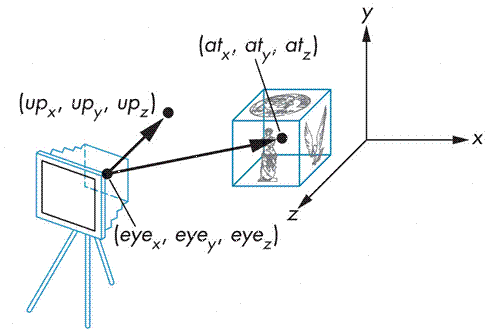
\includegraphics[width=0.4\textwidth, height=0.25\textwidth]{viewport.png}
	\centering
	\caption{Representación gráfica del punto de vista en la escena}
\end{figure}
%
\end{itemize}
\subsubsection{Órbita}
La función para empezar la rotación y darle un sentido, en openGL se conoce como \textbf{getOrbitStartPoint}, esta función recibe como parámetro el ángulo de rotación del planeta, el vector en dónde se almacenarán las coordenadas luego de la rotación, y la posición en $(x,y,z)$ respecto al origen desde la cuál se comienza a realizar la órbita.
%
\lstinputlisting{orbita.c}
%
Esta función realiza el producto de la multiplicación de la matriz de rotación respecto al eje $y$ por el vector de la posición inicial, la cual corresponde al planeta correspondiente.
\subsubsection{loadSkyBox}
La idea detrás de la técnica Skybox, es renderizar un cubo gigante con una textura particular, posicionando la escena y la viewport en el centro\cite{skybox}.\\
Se utilizará la técnica basada en texturas (mapeo de la textura en un cubo), se aplica un tipo especial de textura en el cubo. Esta textura, se crea de forma que para cada cara del cubo, se posicione la textura que le corresponde y que al interior del cubo las esquinas estén perfectamente alineadas, para poder asi crear la sensación de una textura continua.\\
\\
Un ejemplo de esta técnica es la siguiente imagen:
%

\begin{figure}[h!]
	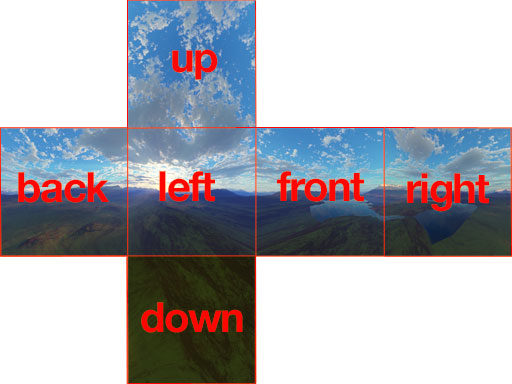
\includegraphics[width=0.4\textwidth, height=0.25\textwidth]{Skybox1.png}
	\centering
	\caption{Ejemplo de una textura que se pueden asignar a las caras de un palco cúbico, con caras etiquetadas}
\end{figure}
%
El procedimiento que se realiza, es cortar cada segmento en una imagen diferente y, en el interior del programa, cada una se trabaja como textura independiente. Posterior a eso, se crea un cubo gigante y se le aplica la textura, el resultado se muestra a continuación:\\
%
\begin{figure}[h!]
	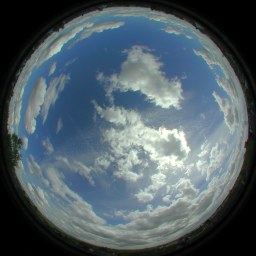
\includegraphics[width=0.4\textwidth, height=0.25\textwidth]{Skybox2.png}
	\centering
	\caption{Ejemplo de una textura para una cúpula celeste hemisférica}
\end{figure}
%
\\
El resultado es un cubo, la aplicación de esta técnica al proyecto es poder darle la forma continua al sistema solar, sin tener un fin a la vista.\\
Se utiliza el formato de imagen (TGA), ya que es la forma más óptima de ahorrar los costos de renderizando\cite{foley}, utilizando un formato de imagen que es de fácil lectura y de una calidad menor.
%
\subsection{Menu de opciones}

Como prototipo, se tienen las siguientes opciones:

\begin{enumerate}
	\item \textbf{Iniciar movimiento}: Inicia la animación de los planetas orbitando.
	\item \textbf{Detener movimiento}: Detiene la animación de los planetas orbitando.
	\item \textbf{Salir}: Salir del sistema solar.
\end{enumerate}
Cabe mencionar que como es un prototipo, aun no se han agregado la totalidad de las funcionalidades mencionadas en los requerimientos, se incorporaron los que están completamente ejecutados y sin fallas, para la entrega final se mostrara el software con la totalidad de los requerimientos aplicados.
\section{Metodología y herramientas a utilizar}
\subsection{Metodología}
La metodología a utilizar es el análisis y diseño estructurado ya que con esta metodología se tiene un orden lógico en los pasos a seguir para el desarrollo correcto del proyecto.
\subsection{Herramientas}
Preliminarmente se tienen las siguientes herramientas para el desarrollo:
\subsubsection{Equipos}
Se posee 2 notebooks con similares características, procesadores Intel core I3 y I5, CPU de 2.4 GHz, 8 Gb de memoria Ram y distribución de Linux Ubuntu 14.04 LTS.
\subsubsection{Herramientas de programación}
Preliminarmente se establecen las siguientes herramientas para la programación, tales como:
\begin{itemize}
 \item Netbeans IDE 8.0.2\\
 	Entre algunas cosas destaca la rápida observación de errores de sintaxis y fácil compilación.
 \item OpenGL\\
 	Principal entorno de desarrollo, para la creación de aplicaciones gráficas portátiles e interactivas en
 	2D y 3D \cite{opengl}.
\end{itemize}
\section{Análisis de resultados}
\subsection{Validación de resultados}
Como se especificó en  la presentación preliminar de la idea, para realizar esta aplicación se toma como base un proyecto anterior del ramo de computación gráfica, el cual se llama "Representación del sistema solar en OpenGL". De este código se toman las funciones principales para generar la representación.\\
En el código se representa Plutón que no se encontraba representado, además se comienza generando todos los planetas alineados tras el Sol para mantener un orden mas lógico en un principio.\\
Se toma como base científica las distancias normalizadas de los planetas y sus velocidades de rotación.
\subsection{Rendimiento preliminar}
En esta etapa de prototipo del proyecto, el equipo de trabajo se enfoca en implementar las funciones más importantes del proyecto base además de aprender sobre la utilización de la herramienta OpenGL. A la base tomada para el desarrollo se le eliminan una serie de funciones que en realidad no serán necesarias por lo tanto esto entregara un código mas compacto y fácil de comprender.\\
Preliminarmente no se identifican problemas relacionados a la presentación en pantalla de la aplicación al ser ejecutada, la velocidad de movimiento (rotación) es más que suficiente para identificar los movimientos de los planetas.\\
El rendimiento gráfico de la aplicación es prudente(por la sencillez), rápido(por como se aprecia) y optimo(por como se realiza).
\subsection{Problemáticas y funciones faltantes}
%
Como se mencionó anteriormente, la función principal que se debe completar es la que da fin al sol, aumentando su radio y su color, transformándose en una gigante roja\cite{far}. De esta manera, absorvera la orbita y los planetas Mercurio y Venus, dejando asi la temperatura de la tierra en mas de 1000º, haciendo asi imposible la vida en la tierra.\\
\\
La función secundaria que se quiere implementar es tener la vista desde cada uno de los planetas, lo cual permitiria tener una perspectiva distinta del fenómeno y de las traslaciones.
\section{Plan de Trabajo}
Se realiza una carta Gantt para darle fechas limites a cada tarea que este proyecto conlleva. Se adjunta para no entorpecer el modelo de este documento y para que la carta Gantt se pueda analizar de mejor manera.
%
\section{Experimentos}
En la imagen se puede observar los planetas alineados, esto muestra el punto de partida del programa.
%
\begin{figure}[h!]
	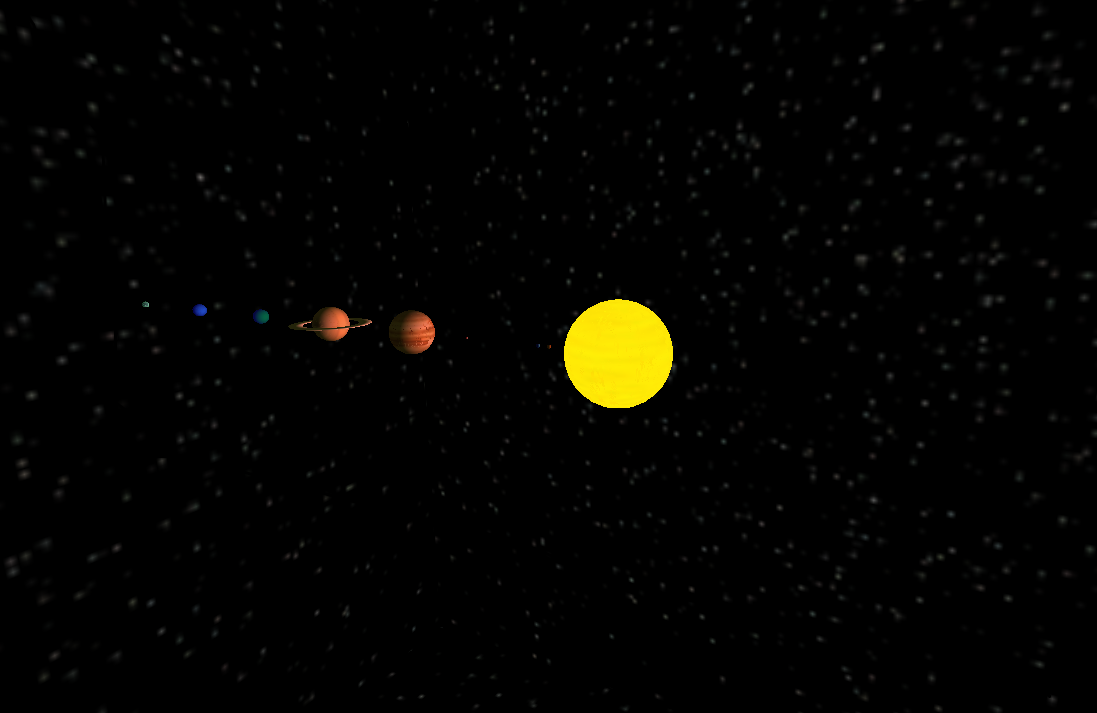
\includegraphics[width=0.4\textwidth, height=0.25\textwidth]{1.png}
	\centering
	\caption{Experimento con las técnicas que se mencionaron aplicadas}
\end{figure}
%
En la imagen se puede observar un momento de la órbita de los planetas, cuando estos ya están orbitando y trasladándose a través de su propia elipse y su propia velocidad.
%
\begin{figure}[h!]
	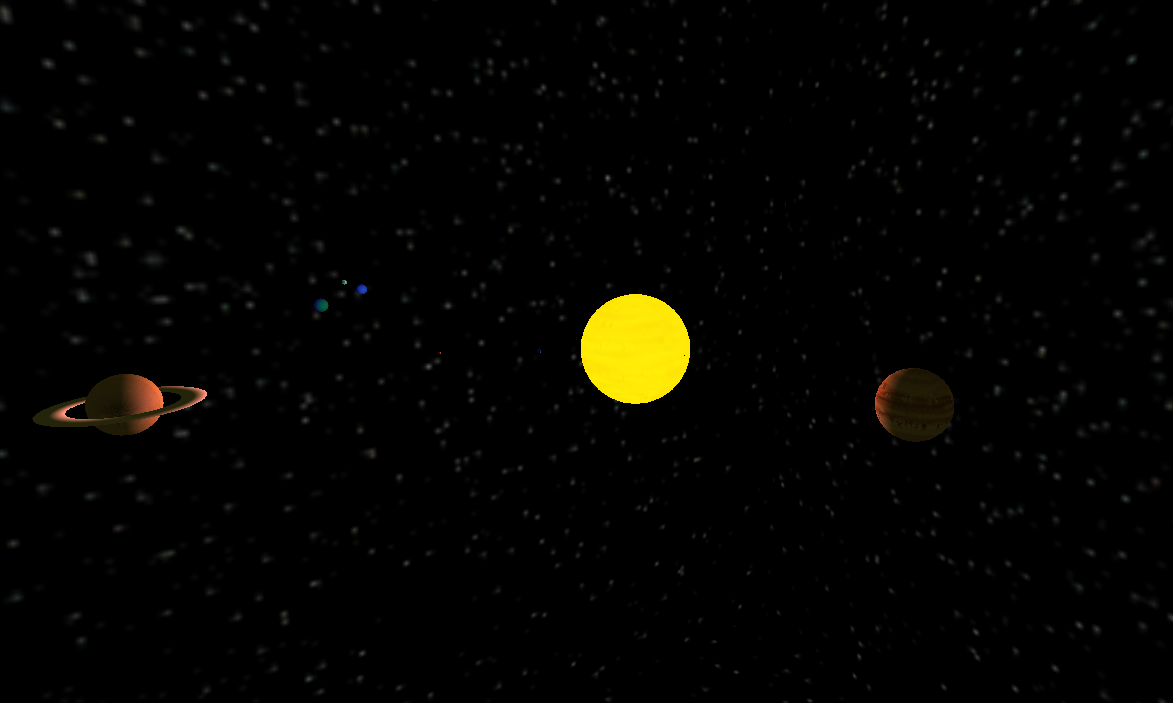
\includegraphics[width=0.4\textwidth, height=0.25\textwidth]{2.png}
	\centering
	\caption{Experimento que muestra las posiciones de los planetas luego de rotaciones}
\end{figure}
%
%
\section{Conclusiones}
%
Como inicio para un buen proyecto, siempre se deben llevar a cabo investigaciones que puedan determinar cual tema abordar y que herramientas utilizar para un optimo desempeño durante este.\\
El tema abordado nos llena de optimismo para trabajar en el, sumado a los conceptos de computación gráfica aprendidos más la investigación pertinente, nos motiva a dar el 100\% de nuestro esfuerzo para hacer de este un gran proyecto.
%
\bibliographystyle{IEEEtran}
\bibliography{bibi}
% that's all folks
\end{document}